% This file is based on the "sig-alternate.tex" V1.9 April 2009
% This file should be compiled with V2.4 of "sig-alternate.cls" April 2009

\documentclass{sig-alternate}

\usepackage{url}
\usepackage{color}
\usepackage{enumerate}
\usepackage{balance}
\permission{}
\CopyrightYear{2013}
%\crdata{0-00000-00-0/00/00}
\begin{document}

\title{Visualization of Music Artist Networks }
\numberofauthors{1}
\author{
\alignauthor
Anonymous
}


\date{11 October 2013}
\maketitle
\begin {abstract}
Our project aims to create a visual network of music artists 
and their relations to other music artists. Data will be obtained 
from a large number of Wikipedia articles using techniques such 
as plain text analysis. An auxiliary database will be developed to 
create structure out of the semi-structured raw data we will receive. 
This will allow for an efficient searching and give way to a faster user interface. 
The user interface will be an application that will use an interactive network 
display that shows the following: the original queried artist, the 
connections that artist has to other artists, and the connections 
of other artists in turn. Visualization of our data is one of 
the main focuses of this project and will be facilitated by our
 interactive network display application, creating an enjoyable and relatively 
simple experience for the user to search our structured database.

\end{abstract}

\section{Overview}
\label{overview}
The goal of this project is to develop an application that will create 
a visual map of a music artist's social network. For example, say you query 
for ``Dr. Dre". The query will display how Dr. Dre is related to Eminem as 
his producer, and to N.W.A as a former member of the group. If you then 
choose ``N.W.A.", the application will explain that N.W.A. is also related to 
 Ice Cube and MC Ren because they are also former members. The goal is 
to ultimately have all of the relations to the original query, in this case Dr. Dre, 
displayed in an interactive graph that the user can use to jump from one 
artist, band, or fact, to another using the information mined from the data. 
Data visualization is the goal of our interactive map. Making it easy 
for the user to query artists and see all of their relations will 
be facilitated by our interactive graphical application. Also, the data domain 
of ``music'' is something almost everyone can relate to, making it 
a good choice for this project; many people can claim to have domain 
expertise in the category of music.

The dataset will be taken from a dump of the English Wikipedia. This implies 
that we will be mining semi-structured data from the wikicode that generates an 
article text. Also, many of the pages contain a subsection called ``Discography'' 
that will need to be mined for this project. To gather the rest of the data, 
plain text searches can be used to find ``produced by", ``collaborated with", 
or ``shared stage with'' relationships, just to name a few. After mining this 
semi-structured data, we will be able to store it as structured data in a database 
that our interactive graph can query. This will be more efficient than the 
application querying the raw data. 


\section{Dataset}
\label{dataset}

The first step in creating our database was the collection of the raw data.
In order to do this, a database ``artistgraph'' was created and a table creation
script was run matching the structure of a wikipedia database. Next, a XML dump from the Wikipedia was downloaded and
mwdumper 1.16, a Java application, was used to extract the data from the XML and load it
into our ``artistgraph'' database. The application contained a graphical user interface
or ``GUI'' which caused some errors. To avoid manipulating the code to resolve these errors,
the command line method of mwdumper was preferred. However, after 246,000 records, the 
Java program would produce an error due to the maximum allowed packet settings in MySQL
being too low\footnote{\url{https://dev.mysql.com/doc/refman/5.1/en/server-system-variables.html#sysvar_max_allowed_packet}}.
This value is small by default in order to catch large, incorrect packets.
This was updated from 16MB to 123MB, resolving the issue.

After running the program
for more than 24 hours, less than 2 million records were loaded. This prompted an 
investigation into why it was loading so slowly. The issue was that the main tables 
(page, revision, and text) have auto increment keys and indices, which were incremented after each insert\footnote{\url{https://www.mediawiki.org/wiki/Manual:MWDumper#Performance_Tips}}.
Because of this, the insert rate was about 13 records per second, which, for
millions of records, is unacceptably slow. To resolve this issue, the tables
were truncated, and the auto increment definition was removed. The indices
of the tables were also removed along with the assignment of primary keys. The altered
script was executed to recreate the tables, and the Java program was run. This resulted
in a loading speed between 600 and 900 records per second. 

This code ran until just shy of 9 million records were loaded. At this point, an unknown error occurred.
Because it is believed that 9 million records is a large majority of the
database, the Java code and the XML file have not been examined yet, since the project is still in an early stage of development. 
With the database loaded, the primary keys were placed in the tables and the indices were recreated.  
The creation of these indices and the assignment of the primary keys only took a couple of hours. 
Considering that the alternative (loading the data with the indices in place) would have taken approximately a week or more,
it was well worth the extra work of removing and then recreating them.
 
Since this database was originally created on a single team member's computer, it was necessary to find a way to copy, 
or move the database to a new location, or at least prove that it could be done for later work.
In order to do this, a MySQL dump was initiated, but failed. This was, perhaps, due to the large size of the database. 
To overcome this, table optimization statements were executed against each table in the ``artistgraph'' database. 
This created separate .idb and .frm files for each table. The .frm file contains the structure of the table, while the 
.idb file contains the data for the table. Copies of these files (more than 100 in total) were made and zipped so that it could 
be shared between the team members. This effectively made the database transferable and proved to be a feasible to move the files in the future.
 
Overall, we have made steady progress on the creation of our database. For the most part, 
all of the data from Wikipedia that we sought to download has been acquired and placed into
our personal database, ``artistgraph". Since we were able to transport the database from one system to another, 
our database should be ready for the next step in our project, code implementation
\ref{code implementation}. 

\section{Architecture and Code Implementation}
\label{architecture and code implementation}

The overall architecture of this project is that of a Master/Worker execution model\cite{Garg:2001:TOA:558986}.
This allows for parallel evaluation of nodes in the graphical representation of data. 
The ``Master'' is a miner which collects and manages the nodes. Nodes will represent 
concepts such as artists, songs, or albums which will ultimately be mapped to Wikipedia 
articles. The ``Workers'' execute the plugins on every node to return more nodes which are 
related to the chosen node. This plugin architecture subscribes modules of code to be 
executed on particular nodes. For example, the ``Infobox'' plugin is meant to be executed 
in ``Artist'' nodes, extracting ``Associated Acts'' from the Wikipedia article of the particular 
artist of that node. Each plugin will find nodes related to the selected node and return 
the type of relationship that the nodes have, be it producer, band member, or other relationship. 
So far, the ``Infobox'' plugin is the only plugin that has been coded. 
Future plugins will further expand the functionallity of the application. Figure \ref{componentdiagram}
shows a component diagram for the current model.

\begin{figure*}[ht!]
\centering
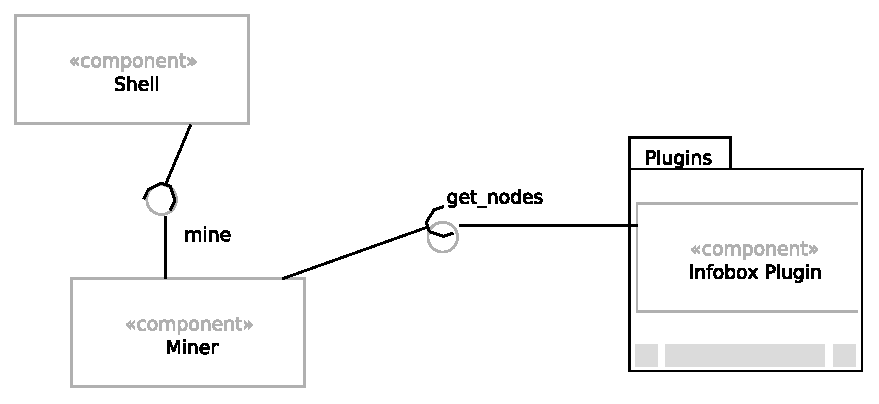
\includegraphics[width=12cm]{ArtistGraph_Architecture.PDF}
\caption{Component Diagram of the ArtistGraph model}
\label{componentdiagram}
\end{figure*}

In order for our application to scale easily if needed, a coding framework needed to be selected. This project 
requires a code that would be easily extensible to parallel computing at a later phase of 
coding while also allowing us to develop portions locally. Initially, Hadoop seemed like 
a viable option, as it is a popular solution for large parallel applications. However, 
this choice would not allow us to execute different pieces of code simultaneously. Because 
Hadoop requires a single algorithm for each reduction step, it was not our choice for this project. 

Our eventual choice of framework for the implementation of our application was PyMW\cite {ieee5161132}. 
This was chosen because it will allow for a ``Generic Interface'' to be used for development. 
This interface can then be transparently switched to a MPI interface for parallel computing and 
benchmarking. It is important to notice that the original code samples for PyMW fell short from
providing information on how to invoke object methods remotely (as opposed to invoking functions
that are part of the standard Python distribution) but these challenges were overcome by
understanding the way this framework splits code for remote execution and applying knowledge
of Python's implementation of Object Oriented Programming.

Future work will include developing the code further to create our node based 
application, making sure that it will work with our database, and deciding on a general 
aesthetic look for the nodes in our application and the associated code required for such nodes. 

{\bf Note: Please disregard the rest of this article as it is just
the template given. Only the above sections were 
for this particular assignment.}


\section{Lessons Learned}
\label{mistakes}

Use this section to describe mistakes you made and corrected (or did
not get a chance to correct including why you didn't).

Graduate students must also include a discussion of how this project
related to current DBSI research.

\section{Current Status and Future Work}
\label{current status}

Use this section to describe the current status of your work
and what else needs to be done.

The next subsection is meant to provide you with some help
in dealing with figures, tables and citations.

\subsection{Tables, Figures, and Citations/References}

Tables, figures, and citations/references in technical
documents need to be presented correctly. As many students
are not familiar with using these objects, here is a quick
guide extracted from the ACM style guide.

\begin{table}
\centering
\caption{Feelings about Issues}
\begin{tabular}{|l|r|l|} \hline
Flavor&Percentage&Comments\\ \hline
Issue 1 &  10\% & Loved it a lot\\ \hline
Issue 2 &  20\% & Disliked it immensely\\ \hline
Issue 3 &  30\% & Didn't care one bit\\ \hline
Issue 4 &  40\% & Duh?\\ \hline
\end{tabular}
\end{table}


First, note that figures in the term paper must be original,
that is, created by the student: please do not cut-and-paste
figures from any other paper you have read. Second, if you
do need to include figures, they should be handled as
demonstrated here. State that Figure \ref{sample graphic} is
a simple illustration used in the ACM Style sample
document. Figures are never below or above the
text. Incidentally, in proper technical writing (for reasons
beyond the scope of this discussion), table captions are
above the table and figure captions are below the figure.

You will find the BibTeX entries needed for many papers being cited,
otherwise you can write your own versions easily and add them to the
$report.bib$ file in the folder. There are many sample bibtex
template files that can be used to model your own references.

The list of all references will be generated in ACMRef
standard style using the \LaTeX{}/BibTeX. Note that you
need to first the following sequence to get the paper
compiled correctly:

\begin{enumerate}
\item {\tt latex} {\em termpaper}
\item {\tt bibtex} {\em termpaper}
\item {\tt latex} {\em termpaper}
\item {\tt latex} {\em termpaper}
\end{enumerate}

\bibliographystyle{abbrv}
\bibliography{termpaper}
% You must have a proper ``.bib'' file
%  and remember to run:
% latex bibtex latex latex
% to resolve all references
\balance
\end{document}
